\chapter{Analysis strategy and background estimation}\label{chap:analysis}

Processes producing SUSY particles have significantly smaller cross sections the most of the SM processes. Therefore, a sophisticated understanding of the relevant production and decay scenarios is needed, in order to separate the potential interesting signal events from the huge amount of SM background. Since this search is targeting SUSY scenarios with bino and wini like NLSPs, finl states with photons and Z bosons are expected, Because the the dileptonic decay of the Z boson is investigated, there are not so much SM background processes leading to this final state. Especially the requirement of a photon and missing transverse momentum $\ptmiss$ reduces most of the background, so that \eg the QCD background is negligible. Leftover are processes producing two same - flavor opposite charge (SFOC) leptons, one photon and missing transverse momentum. The most important ones are $\ttbar(\PGg)$ production, Drell-Yan/$\PZ(\PG)$, $\PZ\PZ$, and $\PW\PZ$ diboson production. More detal can be found in the corresponding sections in \refSec{sec:BKG}.\\
The key strategy of this analysis is, to impose as few as requiremens as necessary, to obtain a inclusive event selection, so that many model scenarios can be investigated. Hence, only the existence of all the expcted final state particles is required, where the Z boson is reconstructed from the two leptons. Therefore, the event selection can be rather loose, including loose requirements on the lepton and photon energies. Not many additional requirements are needed int he following, to obtain a sensitive signal region selection.

\section{Event Selection}
In this first section, the event selection will be explained, including the definitions important for the background prediction, which is based on MC simulation, where the simulation will be handled in dedicated control regions enriched for each group of backgrounds, a validation region to examine the background prediction, and finally a signal region, where two bin counting experiment will be performed. But first, the preselection will be introduced.
\subsection{Preselection}
The preselection acts as a first rough definition of the phase space that is of interest, and rejects inefficient parts of the used triggers. The preselection imposed on the dilepton triggered events is defined as follows:
\begin{itemize}
 \item exactly one SFOC lepton pair ($\Pe\Pe$ or $\PGm\PGm$),
 \item at least one photon,
 \item $\Delta R(\ell_1,\PGg)>0.3$ and $\Delta R(\ell_2,\PGg)>0.3$,
 \item $81\geV<m_{\ell\ell}<101\GeV$.
\end{itemize}
The first two conditions imply the existence of the final state particles, including the definition of the physics objects and lepton pair selection explained in \refSec{sec:reco}. The third requirement reduces contributions of final state radiation photons, that are radiated off by the leptons in the showering process. The last invariant dilepton mass requirement ensures that both leptons originate from a onshell Z boson, and reduces different contributions of SM backgrounds that produce dileptons with an invariant mass not in agreement with a Z boson.
\subsection{Signal region}\label{sec:SRSelection}
The signal region (SR) selection is optimized to maintain high sensitivity for various SUSY scenarios both with electroweak and strong production. For the models considered here, see \refSec{sec:SMS}, the NLSP ($\neutralinoOne$) can decay to a Z boson or a photon in im combination with gravitinos $\gravitino$, that are undectable, leading to missing transverse momentum. Therefore, the requirement of a missing transverse momentum $\ptmiss$ largen than most of the SM background processes are capable to produce, enables a good separation between SM background and SUSY signal. The $\ptmiss$ threshold is not supposed to be to high, to maintain sensitivity to low neutralino masses as well.
Additional high separation power has the stransverse mass $\mtTwo$. Because it yields a good estimate of the NLSP mass, and there is no known SM particle which can decay to photons or a Z boson together with neutrinos creating an momentum imbalance in the detector, $\mtTwo$ on average is much larger for SUSY processes than for SM ones. Both the $\mtTwo$ and $\ptmiss$ distribution of events fulfilling the preselection for the total background and signal points of each model are shown in \refFig{fig:SRvariables}.
\begin{figure}[htb]
 \centering
 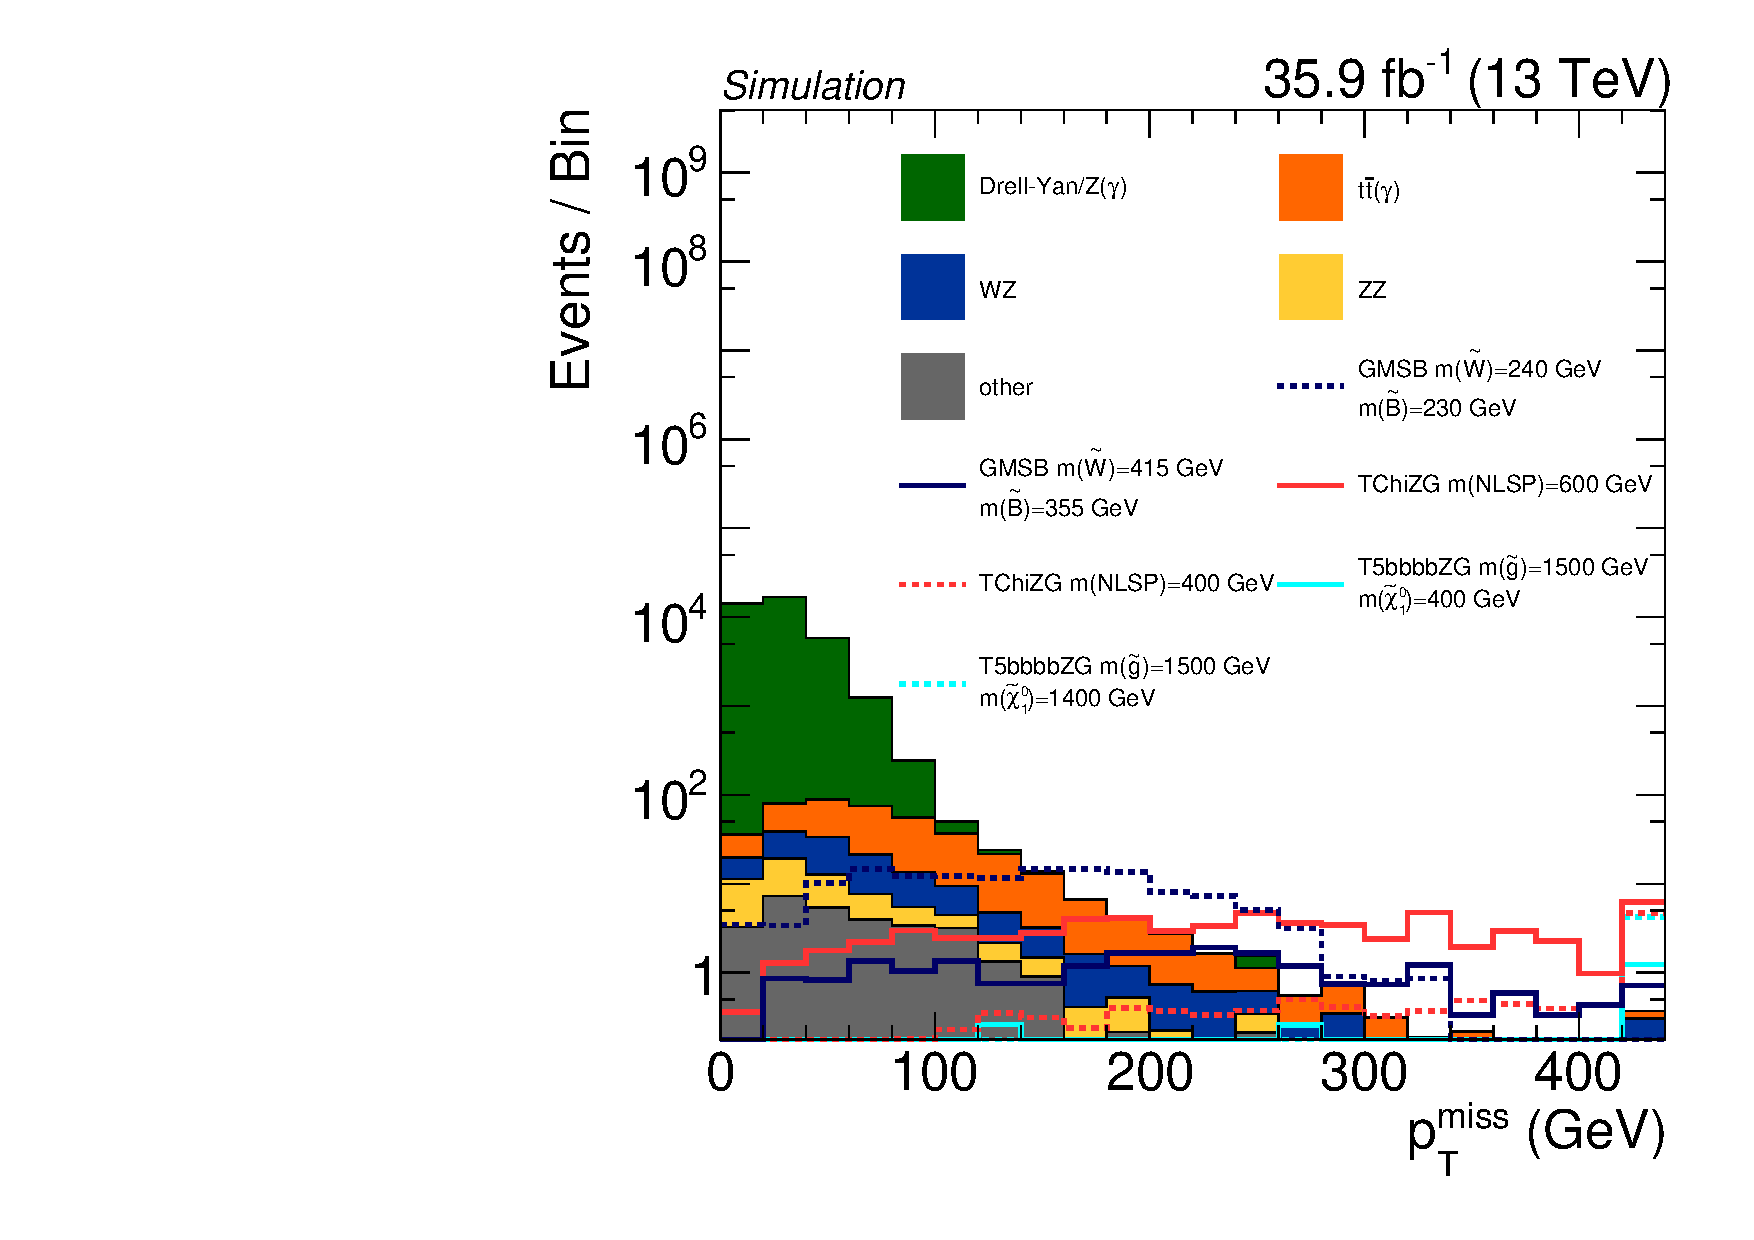
\includegraphics[width=\pairwidth]{figures/mt2/onZ_LL_met_log}
 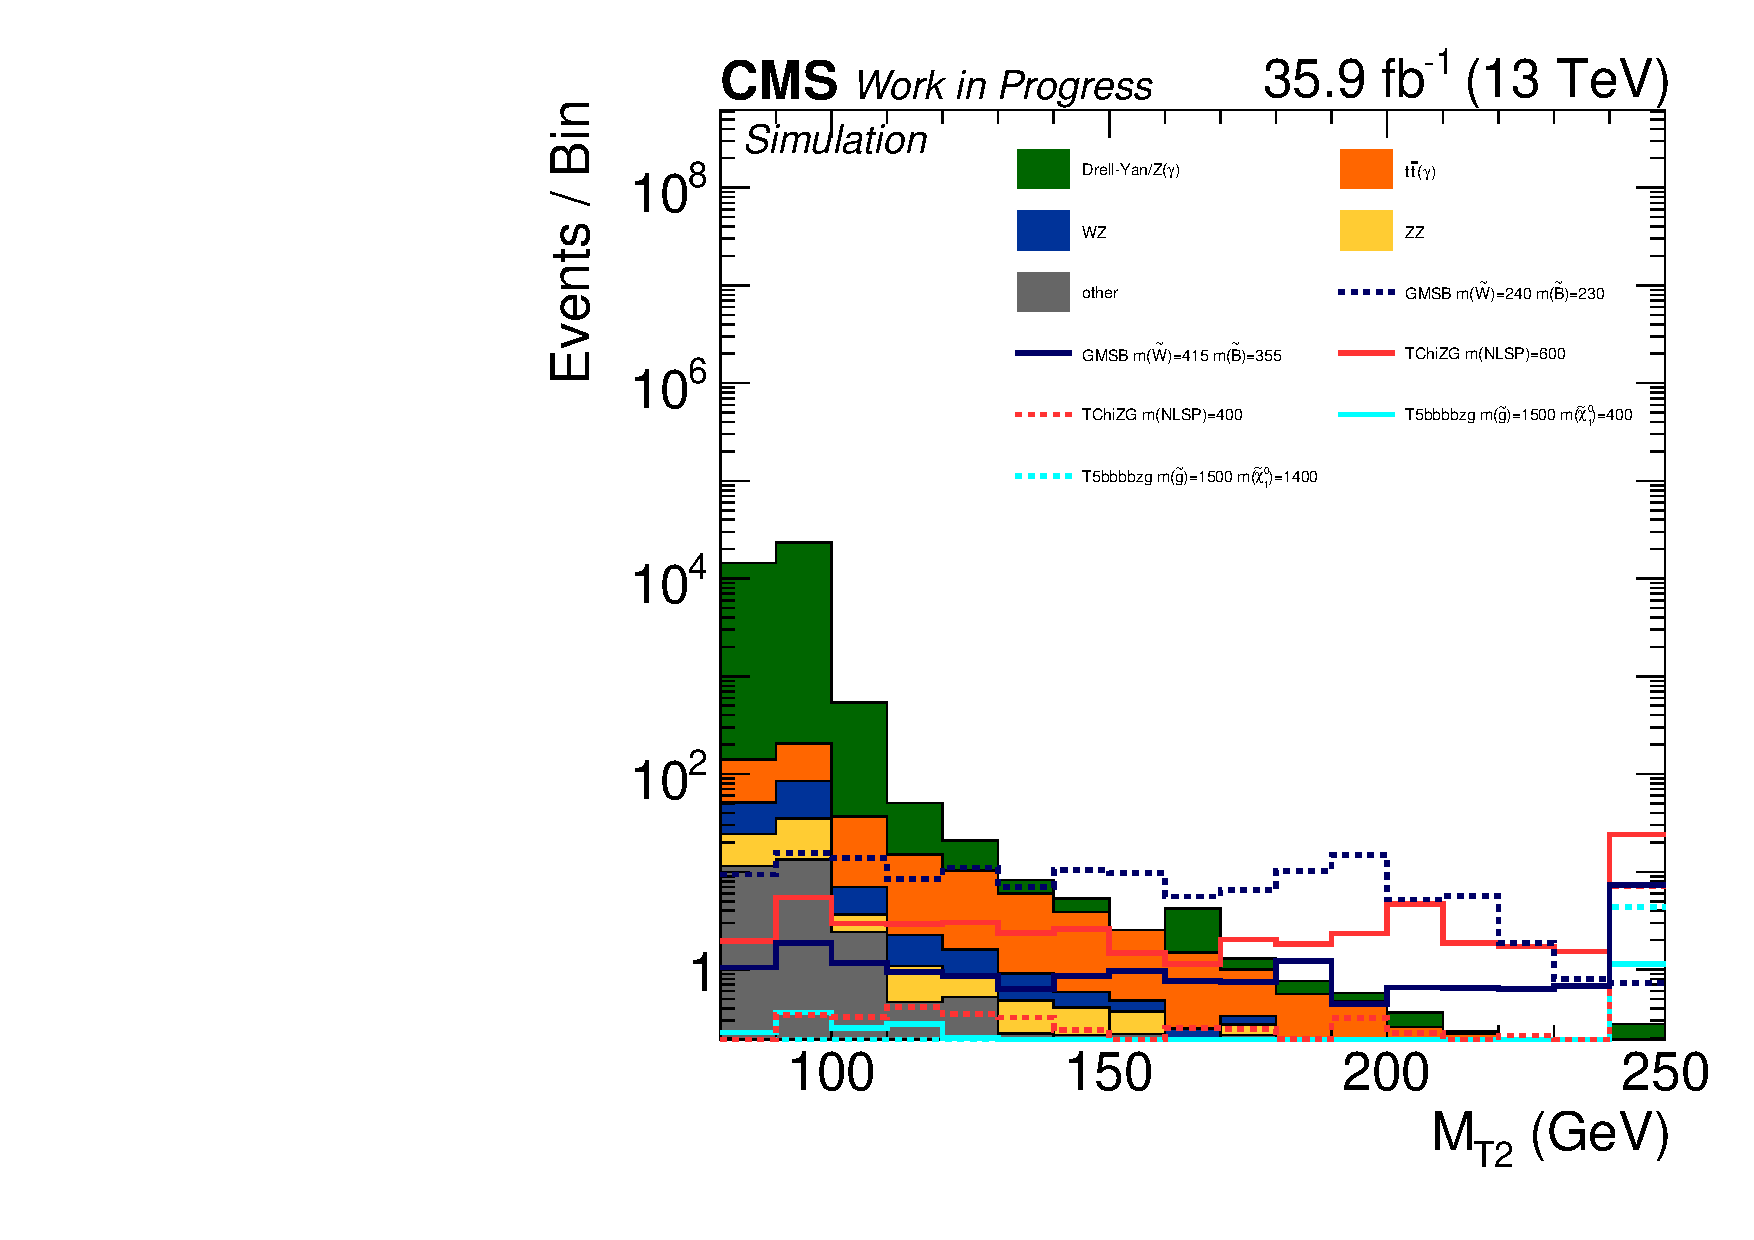
\includegraphics[width=\pairwidth]{figures/mt2/onZ_LL_mt2_log}
 \caption{ToDo}
 \label{fig:SRvariables}
\end{figure}
Hence, the SR is defined trough the following criteria:
\begin{itemize}
 \item $\ptmiss>150\GeV$,
 \item $\mtTwo>100\GeV$.
       
\end{itemize}
The final SR is binned in two search bin in the $\ptmiss$ distribution, one ranging from $150$ to $200\GeV$, and the second from $200\Gev$ to infinity, see \refSec{sec:Results}


\todo{More information to each background, explain here everything.}
\subsection{Control regions}\label{sec:CR}
Different control regions (CRs) are defined for the four main background contributions in order to study and develop a background prediction for the associated background. These CRs are built such, that they are fully orthogonal to the signal region and among each other. The main groups of backgrounds are $\ttbar(\PGg)$, DY/$\PZ(\PGg)$, $\PW\PZ$, and $\PZ\PZ$ production.

\subsubsection*{$\ttbar(\PGg)$ - control region}
To obtain a CR for the $\ttbar(\PGg)$ background with high statistics, the flavor symmetry of the procees is exploited. The two top quarks can decay independently with the same probability to an electron or a muon, resulting in an equal number of same flavor and different flavor final states in case of $\ttbar(\PGg)$ production. Here, the different flavor triggers are needed to guarantee a basis data set with a sufficient amount of events. In addition, the background can be studied in the same high $\ptmiss$ and $\mtTwo$ regions where the SR is defined due to the underlying symmetry. The preselection criteria need to be adjusted, resulting in a CR definition of
\begin{itemize}
 \item exactly one different flavor - opposite charge (DFOC) lepton pair ($\Pe\Pgm$),
 \item at least one photon,
 \item $\Delta R(\ell_1,\PGg)>0.3$ and $\Delta R(\ell_2,\PGg)>0.3$,
\end{itemize}
Of course, the invariant dilepton mass window is removed, since the reconstruced dilepton mass is not in coincidence with the Z boson mass, but has continous distribution different from the top quark mass, because the neutrinos originating from the leptonic top decays are not reconstructed individually and are therefore not considered in the calcuulation. The requirement being responsible for the orthogonality to the SR is the different dilepton composition requirement.
\subsubsection*{Drell-Yan/$\PZ(\PGg)$ - control region}
The Drell-Yan/$\PZ(\PGg)$ background has nearly the same phenomenological topology as the SUSY signal, except for lower missing transverse momentum, since it is mainly due to mismeasurements of jets. Therefore, the $\ptmiss$ distribution of the Drell-Yan/$\PZ(\PGg)$ background is defined by the $\ptmiss$ resolution of the detector and reconstruction. The final control region definition on top of the preselection reads only:
\begin{itemize}
 \item $\ptmiss$<100\GeV.
\end{itemize}
So this region is orthogonal to the SR per definition of the inverted $\ptmiss$ requirement.
\subsubsection*{$\PW\PZ$ - control region}
In order to obtain a high purity $\PW\PZ$ control region, the SFOC dilepton criteria is adjusted such, that the fully leptonic decay of the diboson system is studied. So, as in the preselection, a SFOC lepton pair is required, but the additional lepton veto is removed. Hence, the existence of third lepton, which can be either an electron or an muon, is demanded. This ensures exlusivity between the SR and this CR. Since the $\PW$ boson decays to a lepton and the corresponding neutrino for the selected events, with an additional $\ptmiss$ and $\m_{T}$ requirement, which is calculated using the third lepton, assumed to come from the $\PW$ boson, and $\ptvecmiss$, and is therefore an estimate for the $\PW$ boson mass, a further selection designated for $\PW\PZ$ diboson production is achieved. In the determination of the lepton pair belonging to the decayed Z boson, all combinations fulfilling flavor and charge requirements are tested, and in the case of multiple valid combinations, the combination with the invariant dilepton mass closest to the Z boson mass is chosen. To ensure a selection with a suitable amount of data, because the cross section for diboson production is rather low, the existence of at least photon from the preselection is removed. The final region selection reads:
\begin{itemize}
 \item exactly one SFOC lepton pair ($\Pe\Pe$ or $\PGm\PGm$),
 \item exactly one additional third lepton ($\Pe$ or $\Pgm$),
 \item $\Delta R(\ell_1,\PGg)>0.3$ and $\Delta R(\ell_2,\PGg)>0.3$,
 \item $81\geV<m_{\ell\ell}<101\GeV$,
 \item $\ptmiss>70\GeV$,
 \item $m_{T}(\ptvecmiss,\mathrm{p_{\ell_3}})>50\GeV$.
\end{itemize}
\subsubsection*{$\PZ\PZ$ - control region}
The strategy to achieve a pure $\PZ\PZ$ diboson selection that is not overlapping with the SR selection is very similar to the $\PW\PZ$ CR selection described above. If events are selected, where both $\PZ$ bosons decay leptonically to charged leptons ($\Pe\Pe$ or $\PGm\PGm$), per definition an exclusive control region is obtained. As in the $\PW\PZ$ CR selection, flavor and charge requirements are considered to construct Z boson candidates from the four selected leptons. In cases, where multiple possibilities to reconstruct two Z bosons exist, the possibility with the first Z boson candidate mass closest to the nominal Z boson mass is chosen. The second Z boson candidate has to fulfill a looser mass agreement. Also, the existance of a photon in the event is not required. In total the selection criteria read:
\begin{itemize}
 \item exactly two SFOC lepton pairs ($\Pe\Pe$ or $\PGm\PGm$),
 \item $\Delta R(\ell_1,\PGg)>0.3$ and $\Delta R(\ell_2,\PGg)>0.3$ for the first pair,
 \item $76\geV<m_{\ell\ell}<106\GeV$ for the mass of the first Z boson candidate,
 \item $50\geV<m_{\ell\ell}<130\GeV$ for the mass of the second Z boson candidate.
\end{itemize}
\subsubsection{Validation region}
An additional validation region (VR) is determined, where the developed background predictions are verified by perfoming data - prediction comparisons. Therefore, it is convinient to choose the VR in phasespace close to the SR. This is achievied by applying the same selection requirements as for the SR, but either the $\ptmiss$ requirement, or the $\mtTwo$ requirement needs to fail. Hence, the VR is a sideband to the SR. The VR may also not overlap with the DY/$\PZ(\PGg)$ CR, thus a minimal $\ptmiss$ requirement needs to be imposed. The selection requirements for the VR in addition to the preselection are the following:
\begin{itemize}
 \item $\ptmiss>100\GeV$,
 \item either $\ptmiss<150\GeV$ or $\mtTwo>100\GeV$.
\end{itemize}
\\
A visualization of the signal, validation, and DY/$\PZ(\PGg)$ control region definitions in the $\mtTwo$-$\ptmiss$ plane can be found in \refFig{fig:Regions}. Two dimensional histograms for the number of expected events motivating the region definitions are shown in \refFig{fig:Regions2} for the all background processes, and each one benchmark point for all three considered signal models.
\begin{figure}[htb]
 \centering
 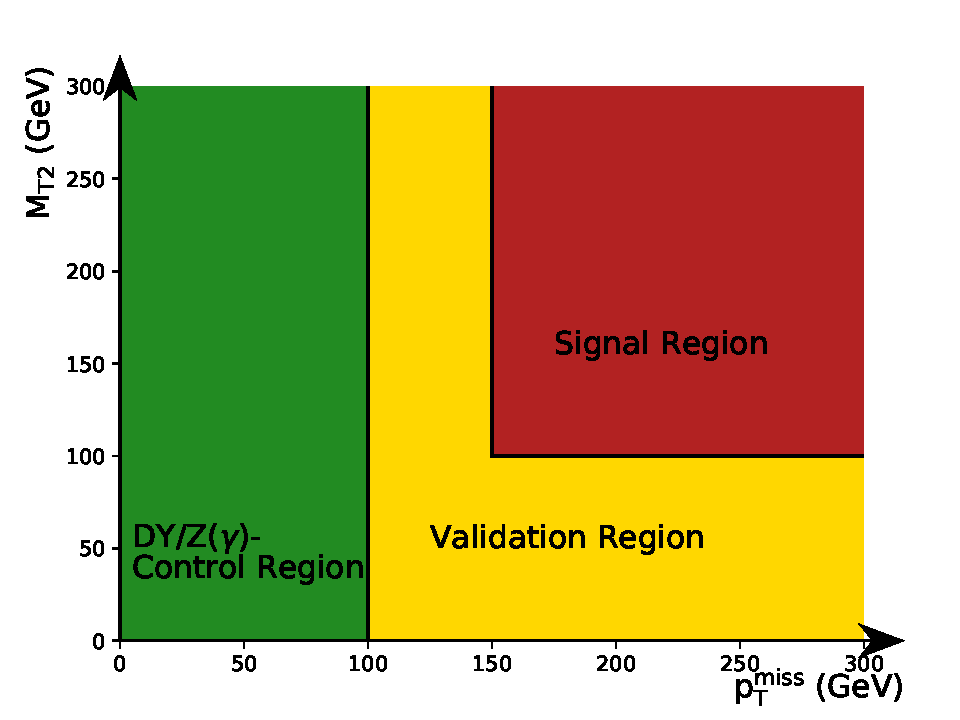
\includegraphics[width=\pairwidth]{figures/figures/regions}
 \caption{Visualization of the definition of the signal, validation and DY/$\PZ(\PGg)$ control region in the $\mtTwo$-$\ptmiss$ plane.}
 \label{fig:Regions}
\end{figure}
These distributions show also specific feautures of the considered signal models regarding the important kinematic observables. Because the \texttt{TChiZG} model is a one parameter scan, and the only free paramater is the NLSP mass, which directly determines the maximum amount of transverse momentum for the decay products, ans thus directly the boson $\pt$ and the $\ptmiss$ due to the gravitinos. Thus, $\ptmiss$ and $\mtTwo$ calculated from the bosons and $\ptmiss$ are strongly correlated per definition. Also, the endpoints of the $\ptmiss$ and $\mtTwo$ distributions are of the same order, and coincide with the NLSP mass. In case of the strong SMS, this is not directly the case. Since this is a two dimensional pramater scan, the event kinematic depends on the mass difference between the gluino and the NLSP mass, as discussed in \refSec{SMS}. In cases where the mass difference is small, the kinemtics evolve similar as for the EWK SMS, while for larger mass differences, as shown in \refFig{fig:Regions2}, the correlation between $\mtTwo$ and $\ptmiss$ is much weaker and the distributions are much broader. The distributions of the GMSB model behave like a mixture of the two SMSs, depending on the wino and bino masses.\\
And most importantly, the signal events mainly populate the SR, with small contributions in the CRs and the VR, while the majority of the background events contribute to the DY/$\PZ(\PGg)$ CR and a minor part to the VR. Only a minority contributes to the SR, as it is desired. So in total a good separation between background and signal is achieved.

\begin{figure}[htb]
 \centering
 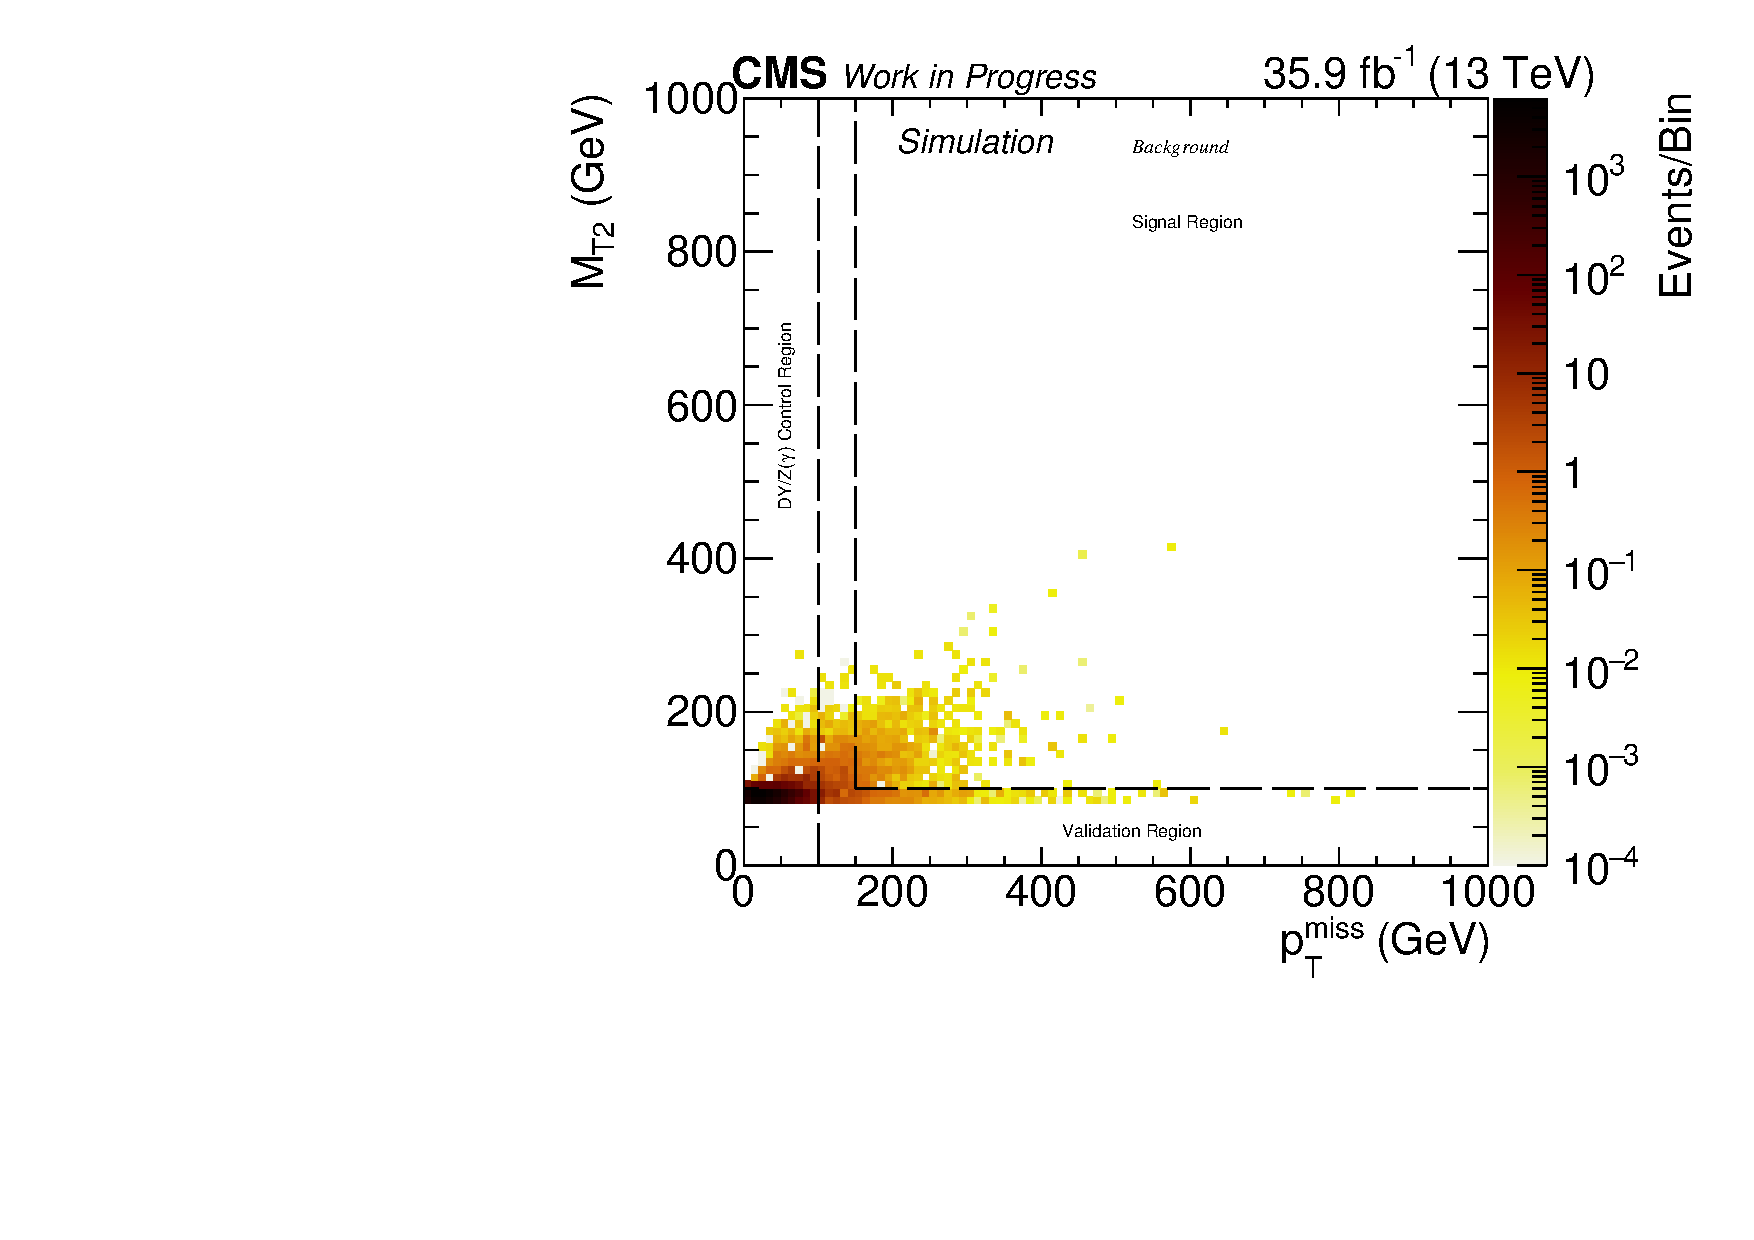
\includegraphics[width=\pairwidth]{figures/plots_2d/DataMC_sameHistograms_LL+signal_onZ__LL__MetMt2_bkg_}
 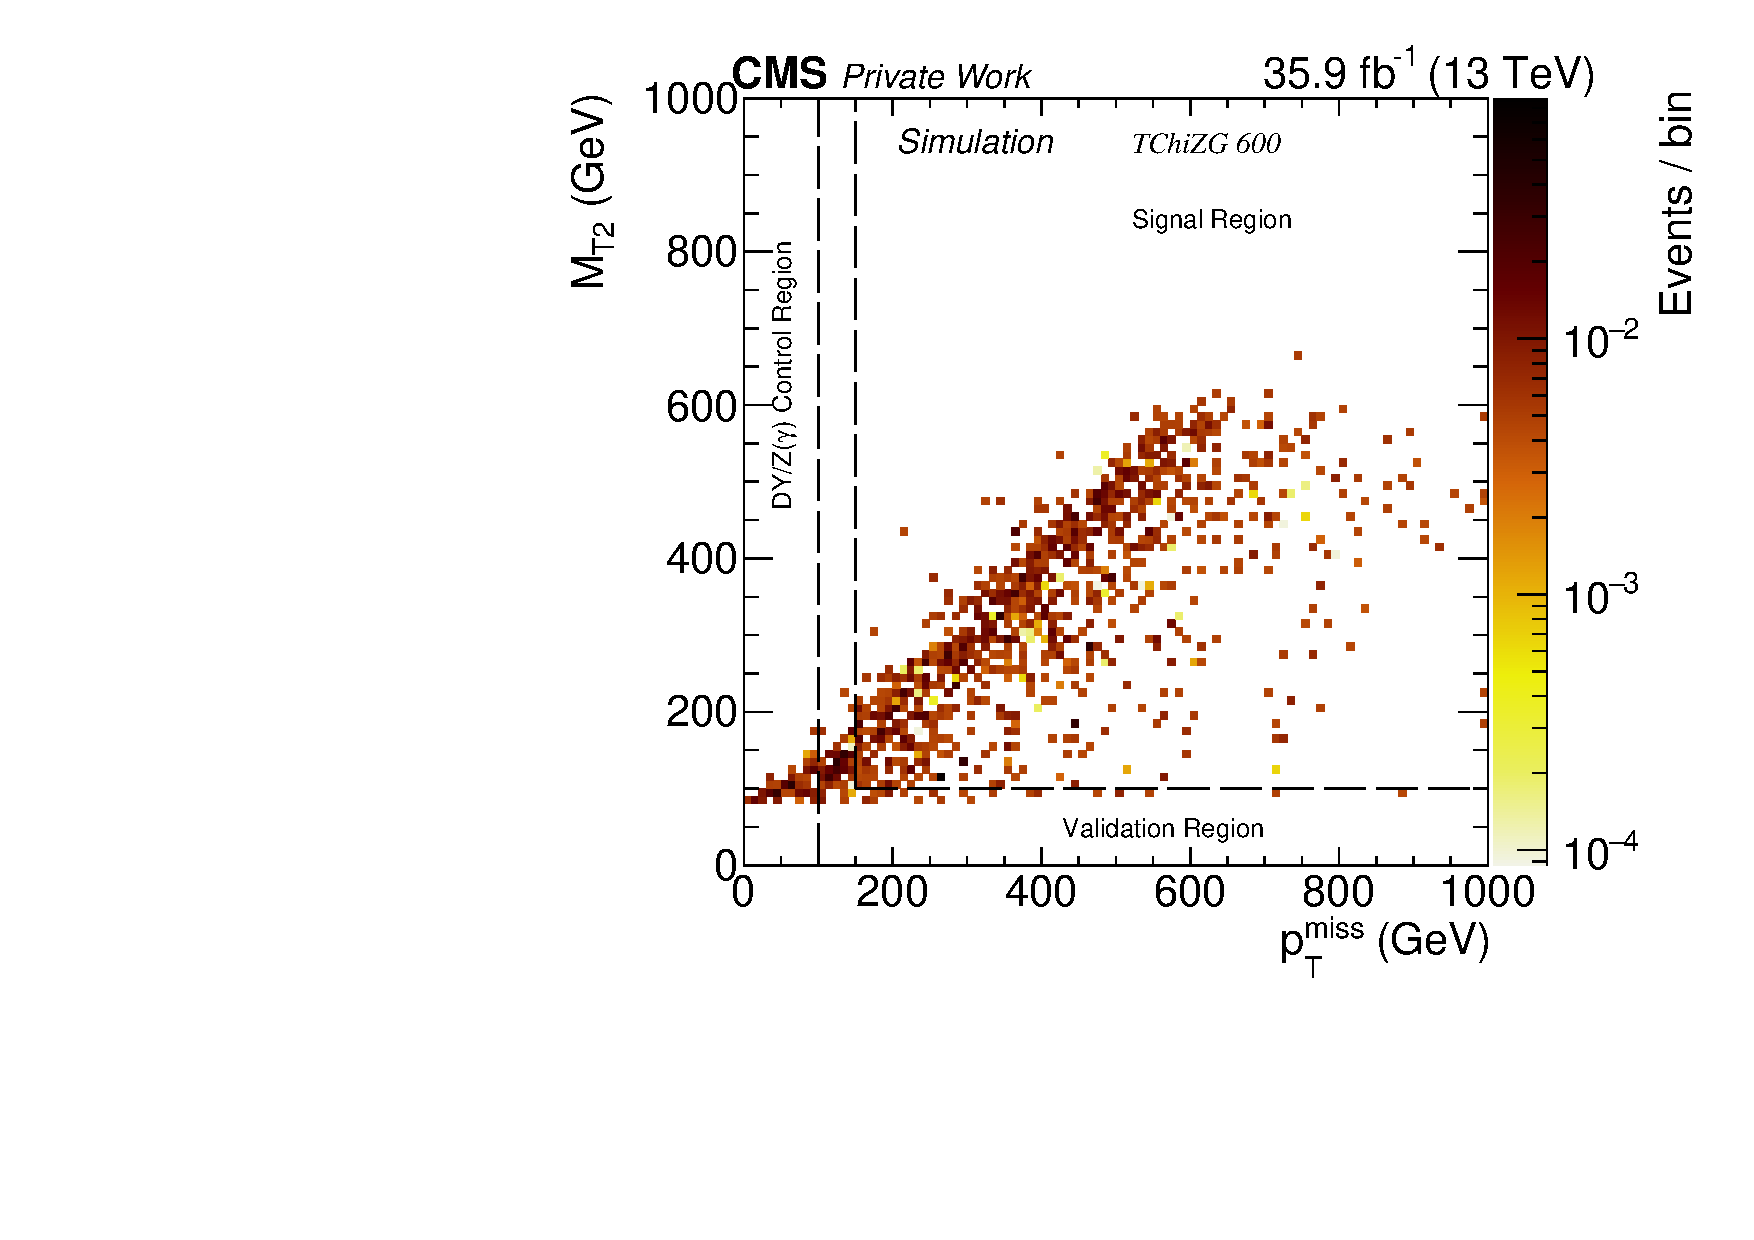
\includegraphics[width=\pairwidth]{figures/plots_2d/DataMC_sameHistograms_LL+signal_onZ__LL__MetMt2_SIG_tching600_}\\
 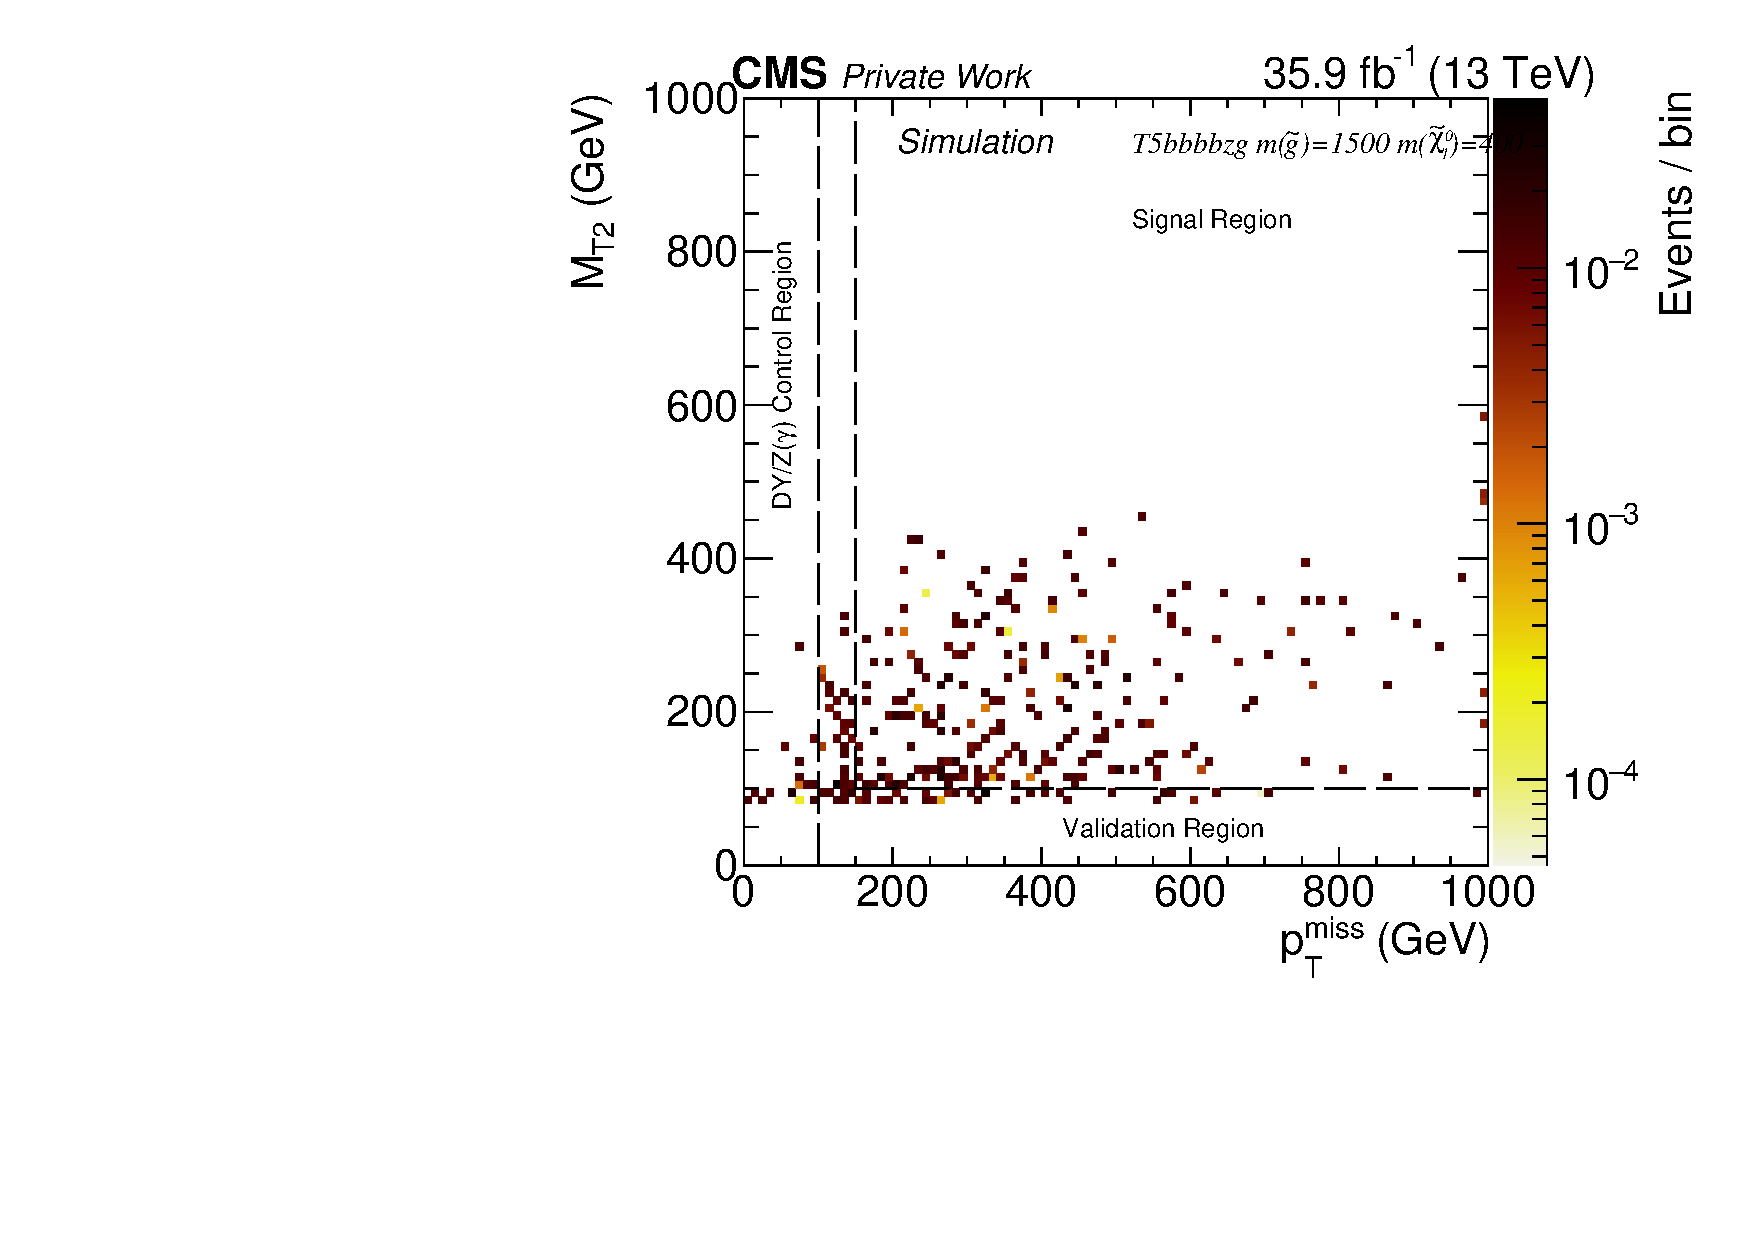
\includegraphics[width=\pairwidth]{figures/plots_2d/DataMC_sameHistograms_LL+signal_onZ__LL__MetMt2_SIG_t5bbbbzg_1500_400_}
 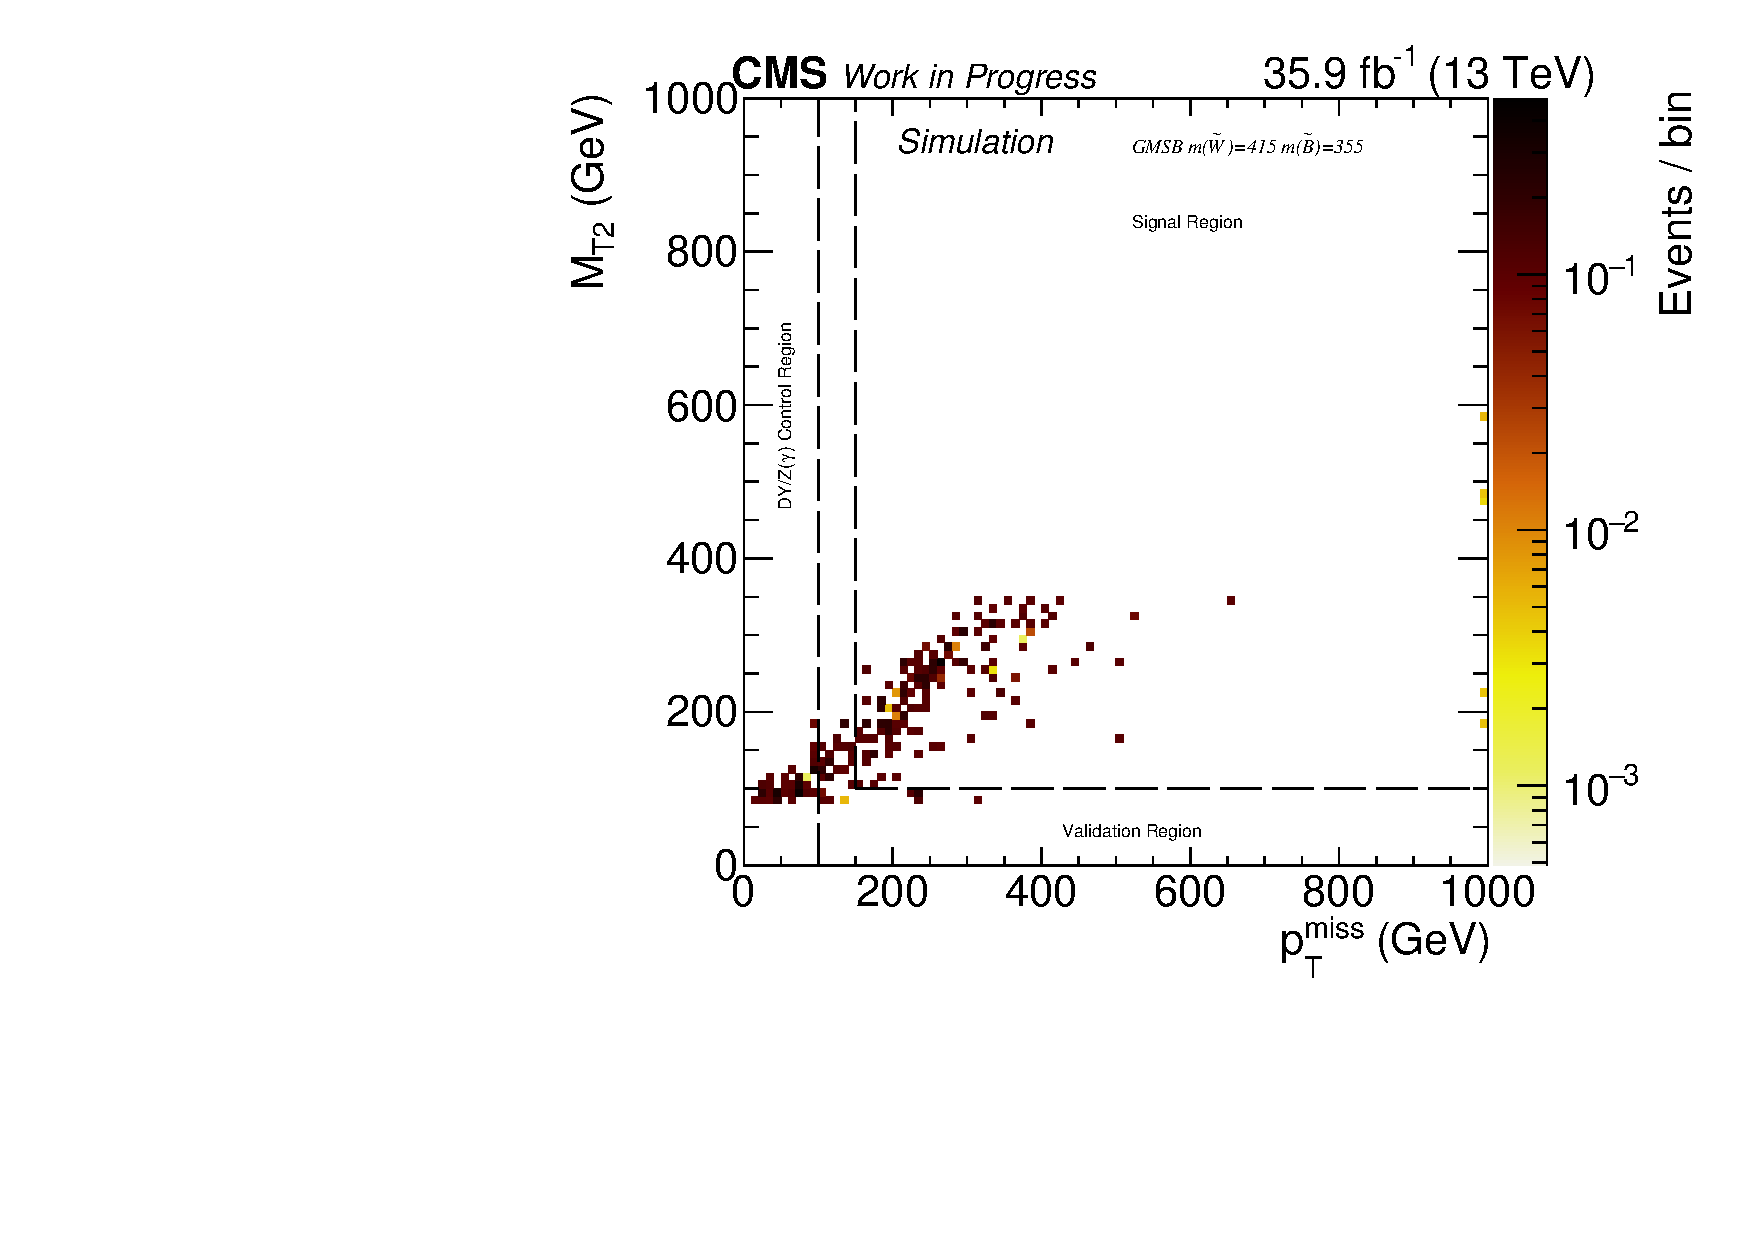
\includegraphics[width=\pairwidth]{figures/plots_2d/DataMC_sameHistograms_LL+signal_onZ__LL__MetMt2_SIG_gmsb_415_355_}
 \caption{Distribution of the total number of expected background events in the $\mtTwo$-$\ptmiss$ plane (upper left). Distributions for the number of expected signal events for the \texttt{TChiZG} SMS with an NLSP mass of $600\GeV$ (upper right), the \texttt{T5bbbbZG} SMS with a gluino mass of $1.5\TeV$ and a neutralino mass of $400\GeV$ (bottom left), and the GMSB model with $m(\widetilde{W}=455\GeV)$ and $m(\widetilde{B}=355\GeV)$ (bottom right).}
 \label{fig:Regions2}
\end{figure}



\section{Background Estimation}\label{sec:BKG}
In this section the used background estimation methods are introduced, including the study of systematic effects. The total background is composited of $\ttbar(\PGg)$ production, Drell-Yan and $\PZ(\PGg)$ events, $\PW\PZ$ and $\PZ\PZ$ diboson production, and a remaining group of backgrounds, composited of \eg singletop and triboson production (See \refSec{Simulation} and \refSec{sec:CR}). The relative amount of backgrounds contributing to the two SR bins are depicted in \refFig{fig:PieCharts}. The most dominating background is $\ttbar(\PGg)$, followed by $\PW\PZ$, $\PZ\PZ$, and Drell-Yan/$\PZ(\PGg)$.\\
The leptonic decays of the top pairs generated in association with a photon significantly contribute to the SR, because the final state signatures appear very similiar to those of the SUSY models and the cross section is very high. If both W bosons decay leptonically, a SFOC lepton pair in connection with neutrinos are produced, that generate a large amount of $\ptmiss$ in the detector. Also real photons can be produced in the hard interaction, or can be radiated off in the initial or the final state by the charged participating particles. Since the total mass of the top pair cannot be reconstruced due to the momentum imbalance, there is a suffienct probability to measure a invariant dilepton mass close to the Z boson mass.\\
In the Drell-Yan process, in context with FSR or ISR, and in $\PZ\PGg$ production, directly a on-shell Z boson is produced, thus the $\m_{\ell\ell}$ requiremet for the SR is fulfilled. Although a photon is also produced, ths background does not contribute significantly to the SR, because only nongenuine $\ptmiss$ is generated in the process due to mismeasurements and therefore the $\ptmiss$ distribution drops steeply.\\
$\PW\PZ$ production is also an important background, since the $\PW$ boson can decay leptonically and therefore can generate a sufficient amount of genuie $\ptmiss$ to pass the SR requirements. While a photon can be generated in all possible radiation processes, an additional electron or jet originating from the $\PW$ boson can fake a photon signature in the detector. In cases of real photons, the additional lepton can also be lost in the reconstruction.\\
Lastly, the $\PZ\PZ$ event signature can be very similar to the one expected from various SUSY signals. One boson can decay to a pair of charged leptons, while the other decays to neutrinos leading to a large amount of $\ptmiss$ in the event. Together with FSR or ISR of a photon, it mimics the signal topology in many ways.\\
If the different background processes are compared, the diboson processes may have a more similar event kinematic than the $\ttbar(\PGg)$ process, but due to the lower diboson cross sections, and the small branching fraction for a $\PZ$ or $\PW$ boson to decay to charged leptons, the $\ttbar(\PGg)$ background dominates the other contributions.\\

\begin{figure}[htb]
 \centering
 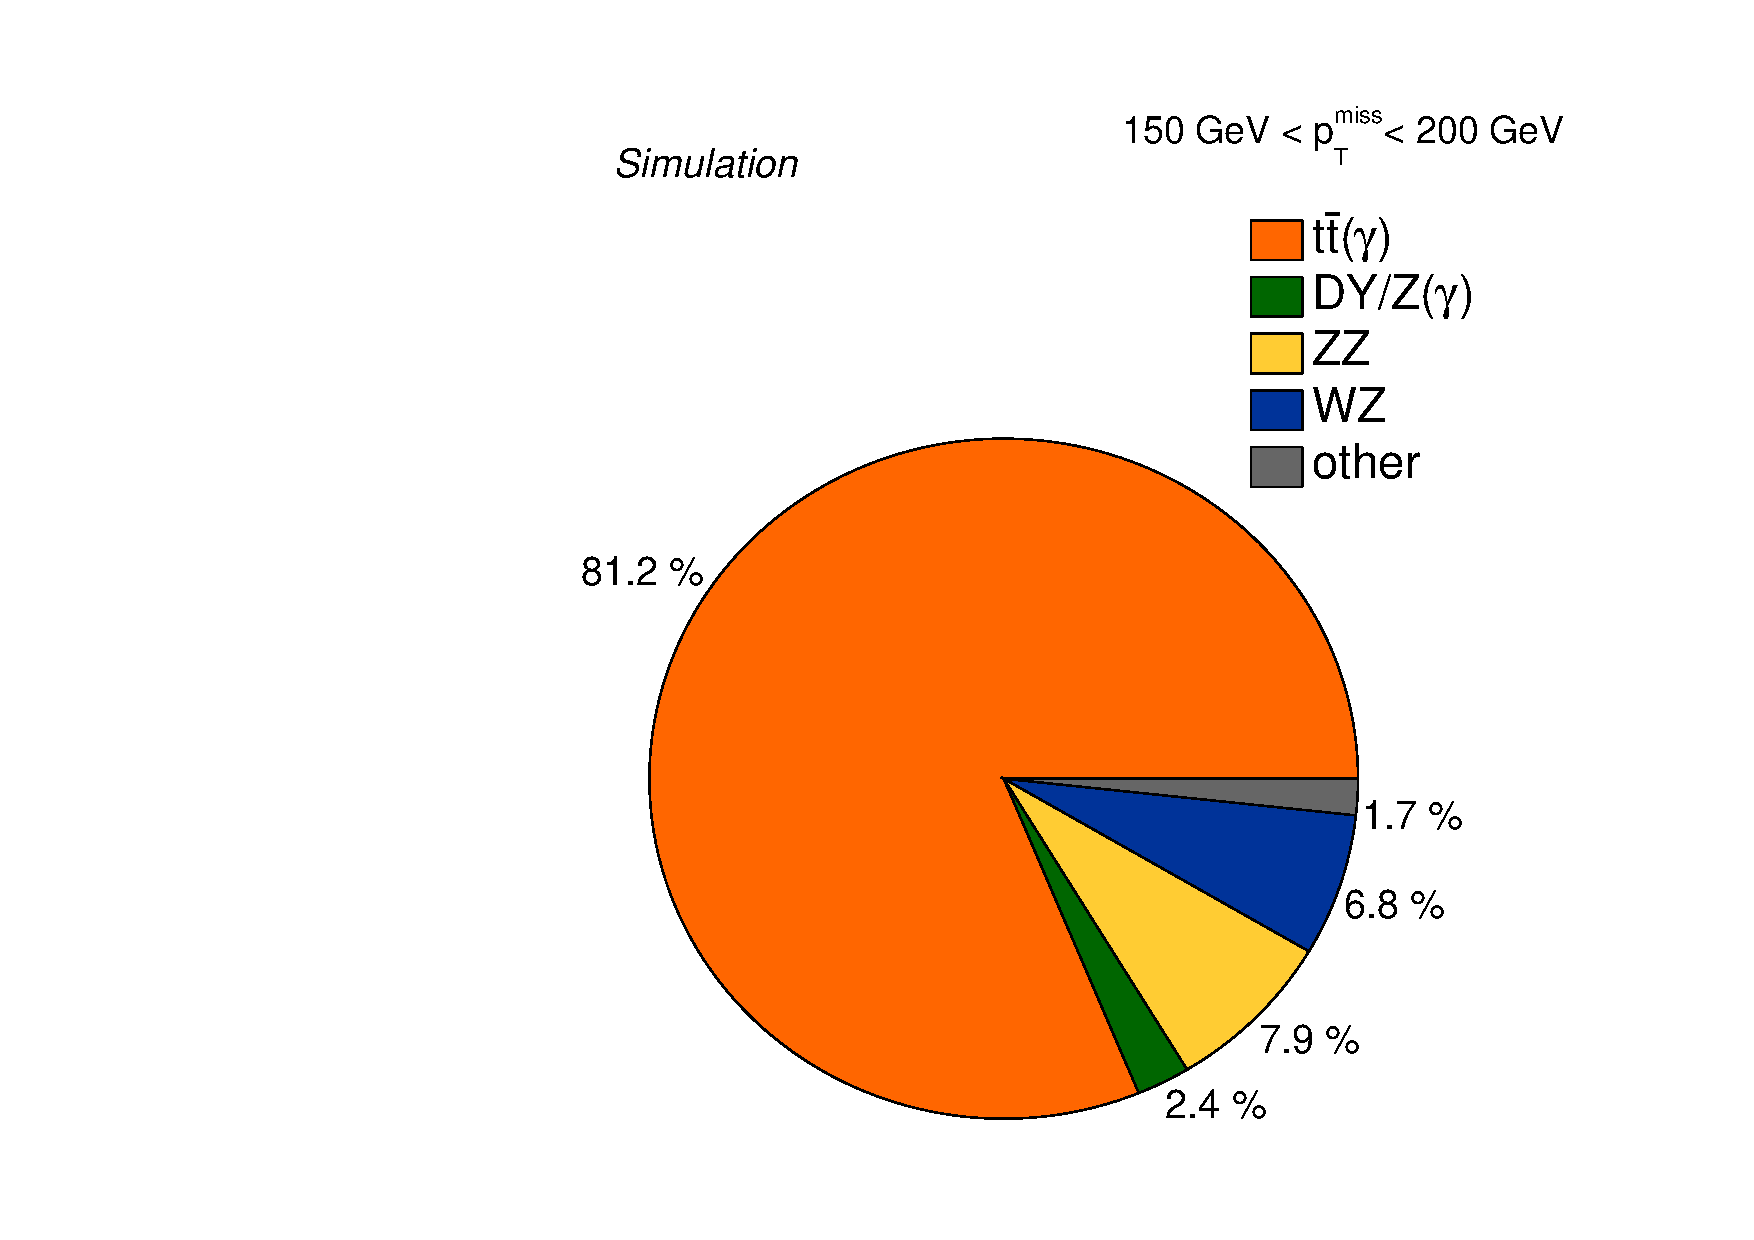
\includegraphics[width=\pairwidth]{figures/figures/pie1}
 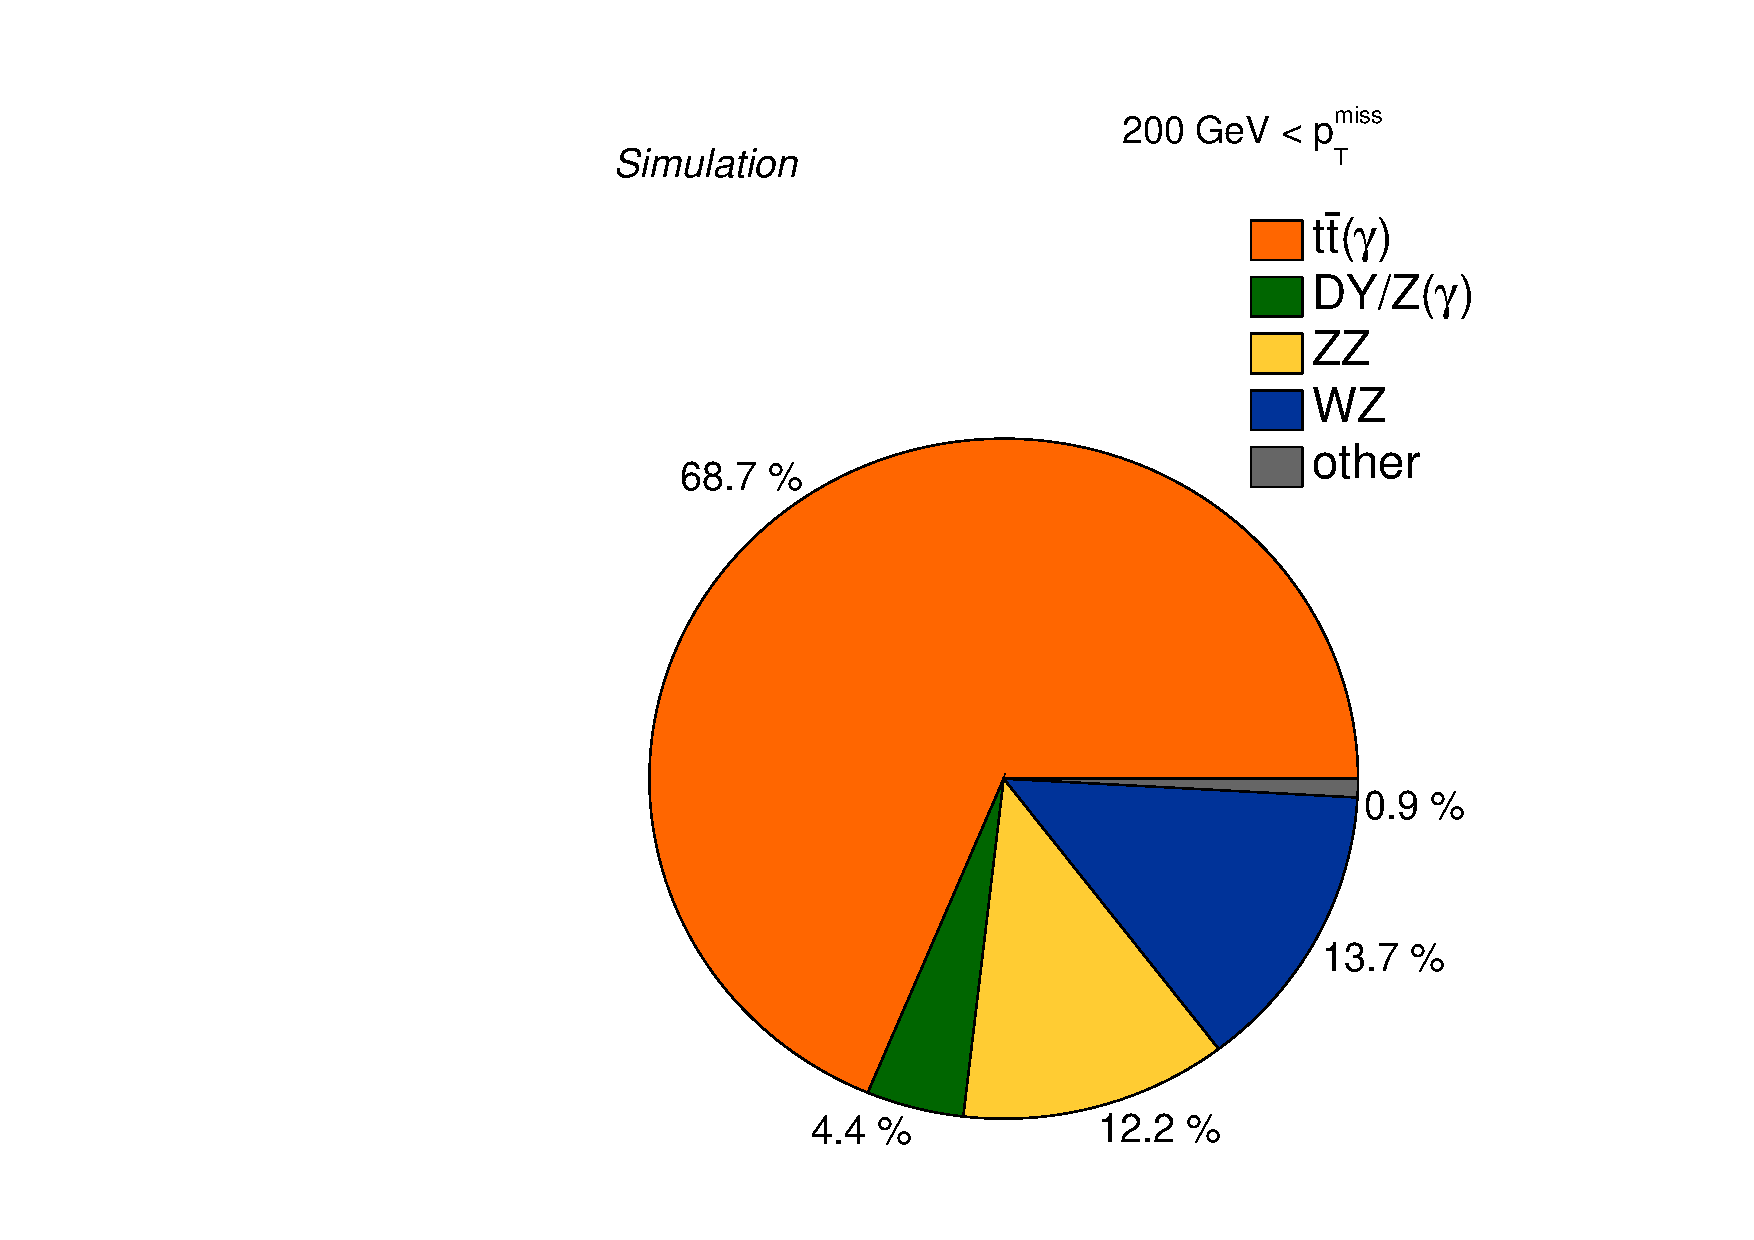
\includegraphics[width=\pairwidth]{figures/figures/pie2}
 \caption{Relative amounts for all group of considered backgrounds for the two search bins in the SR.}
 \label{fig:PieCharts}
\end{figure}
The strategy to perform a sophisticated background prediction is based on the MC simulation for all backgrounds. As mentioned in \refSec{CR}, different CRs are developed, which are enriched with corresponding background events. In those CRs, scale factors (SF) $\alpha_i$ are calculated by scaling the total simulation to the measured data yield. Contributions of other backgrounds in the distinct CR are considered in the calculation by fixing them, thus only one background is scaled. The SFs are calculated via the following formula:
\begin{align}
 1                        & = \frac{\#Data}{#FixedBackground+\alpha_i\cdot\#BackgroundToScale} \\
 \Longrightarrow \alpha_i & = \frac{\#Data-\#FixedBackground}{\#BackgroundToScale}.            
\end{align}
Due to the used method, which is performed similar in every CR, possible uncertainties in the normalization cancel, only uncertainties in the shape need to be considered, see~\refSec{sec:Syst}. The uncertainty arising from the SF calculation is purely of statistical origin, and is calculated via error propagation
\begin{equation}
 \sigma_{\alpha_i}^2 = \sigma_{D}^2 \cdot \left(\frac{D}{B}\right)^2 + \sigma_{F}^2 \cdot \left(\frac{F}{B}\right)^2 + \sigma_{B}^2 \cdot \left(\frac{D-F}{B^2}\right)^2,
\end{equation}
where $B=\#BackgroundToScale$, $F=\#FixedBackground$, $D=\#Data$, and $\sigma_i$ the corresponding statistical uncertainties. These are assumed to be uncorellated Poissonian uncertainties. Since the event yields are high enough, the uncertainties can be calculated via $\sigma_i=\sqrt{N_i}$, where $N$ is the associated total integral in the selection. In the case of MC simulation, for the calculation of the SF the normalized event yield is used, whereas in the error calculation the pure MC event count is considered to reflect the underlying precision of the simulation. These method is referred to as "integral method" in the following.\\
After determining all SFs, the background prediction will be tested in the VR. Therefore, the simulated backgrounds in the VR will be scaled accordingly, and the result will be investigated, see \refSec{sec:Validation}.
\\
To study a possible bias of not well modeled observables in the simulation, additional cross checks are performed. Similar to the SF calculation in the integral method, SFs are determined via $\Chi^2$ minimization in the same CR. Thus, this method is somewhat correlated to the method explained above, but enables the possibility to study influences of different distributions in different binnings.


\subsection{Top pair production in association with a photon}\label{sec:ttbar}


\begin{figure}[htb]
 \centering
 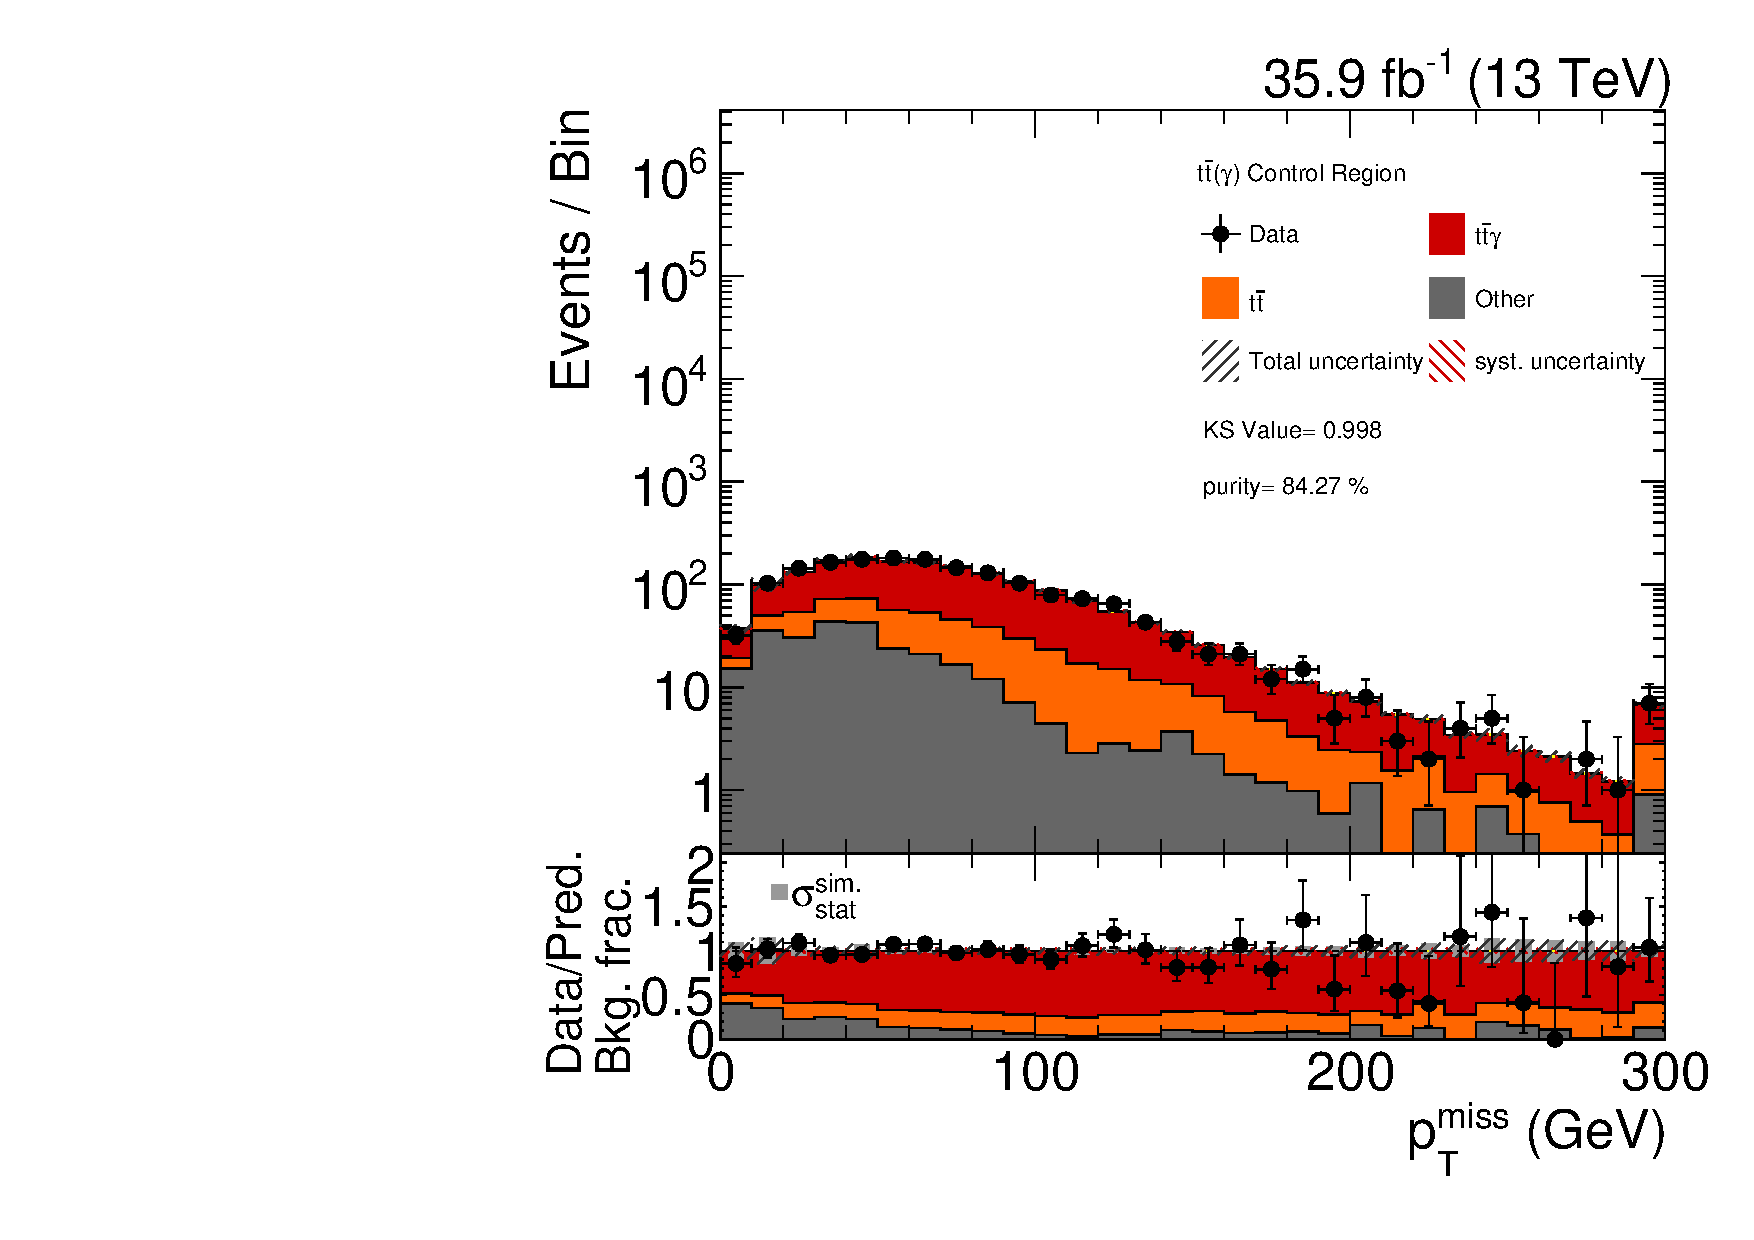
\includegraphics[width=\pairwidth]{figures/plots_CR_tt/CRTT_EM_nom_met_log}
 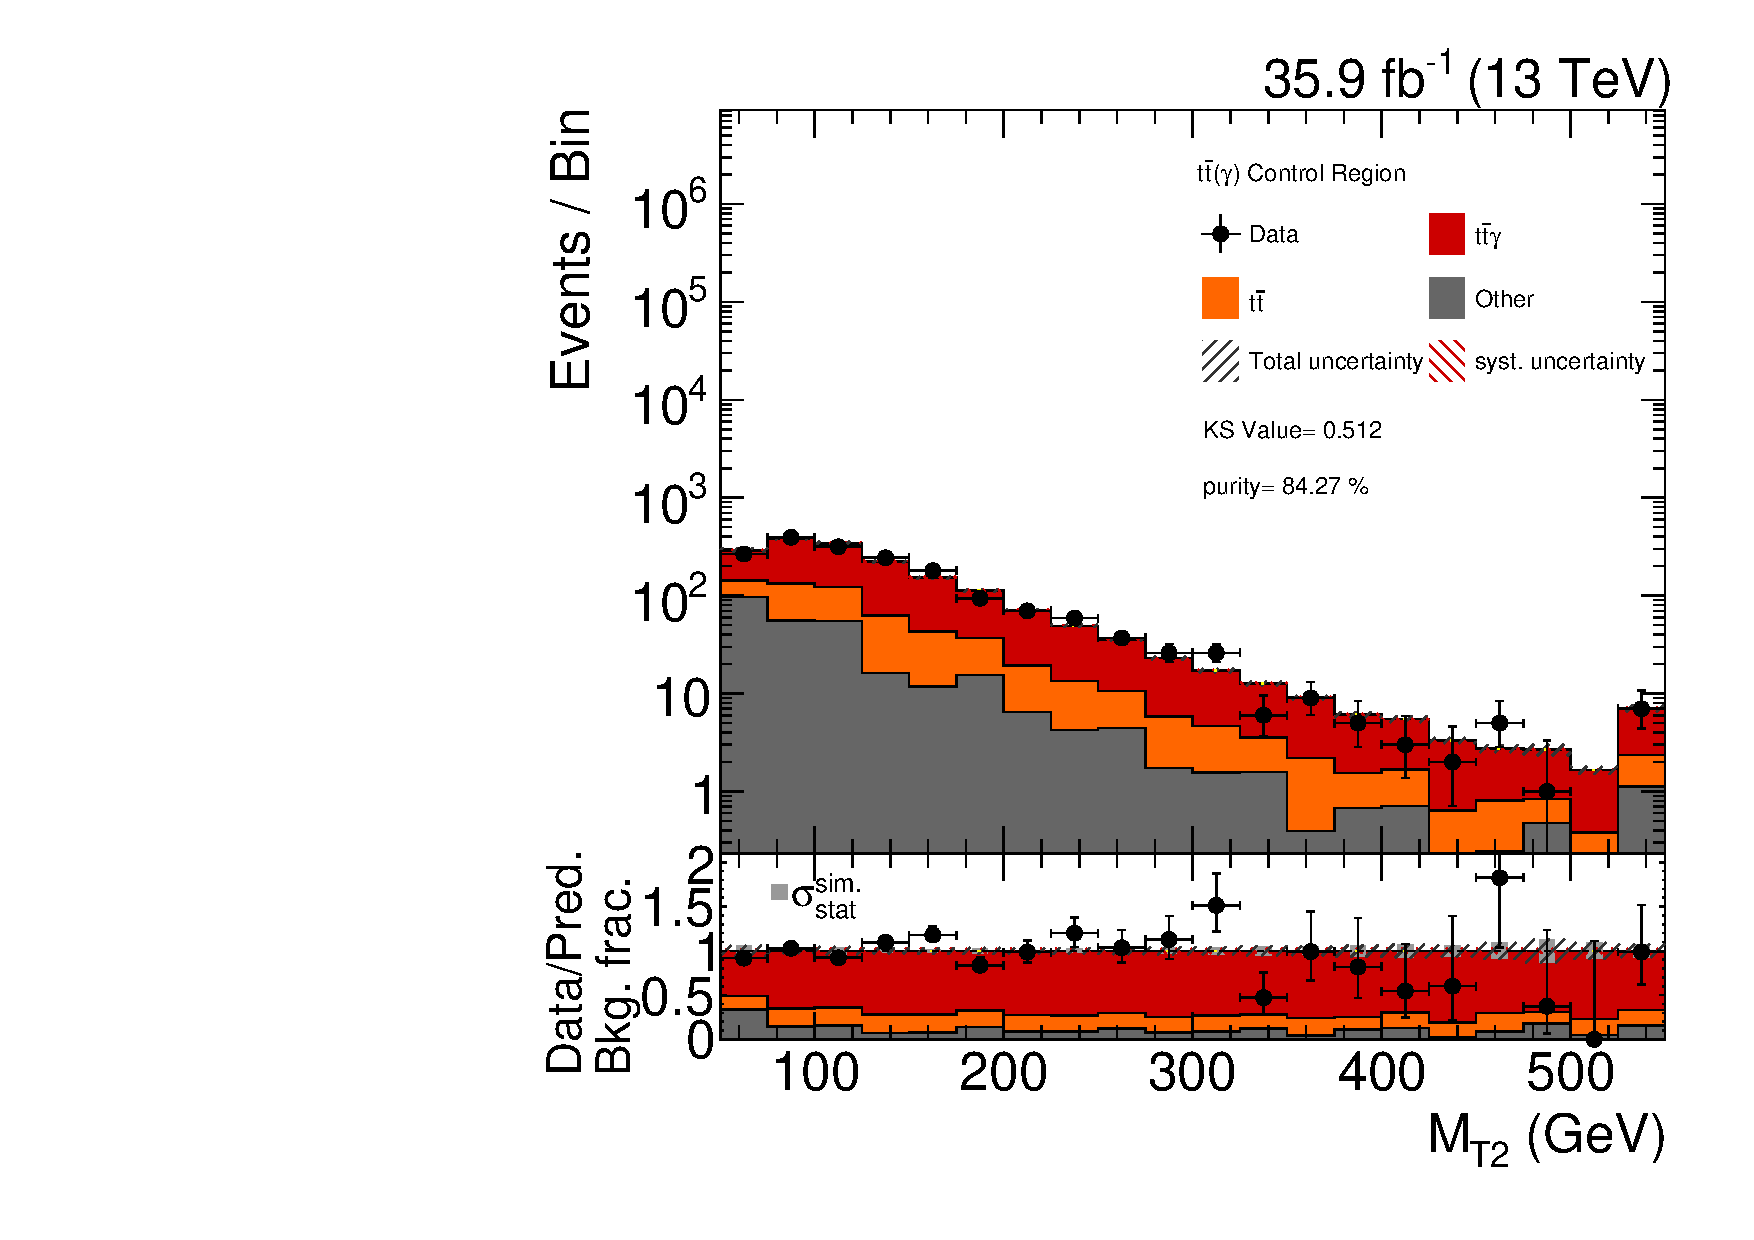
\includegraphics[width=\pairwidth]{figures/plots_CR_tt/CRTT_EM_nom_mt2_log}
 \caption{ToDo}
 \label{fig:TTCR}
\end{figure}


\subsection{Drell-Yan and $\PZ\PGg$ diboson production}
\subsection{$\PZ\PZ$ diboson production}
\subsection{$\PW\PZ$ diboson production}
\subsection{Other standard model backgrounds}
\subsection{Validation of the background estimation}\label{sec:Validation}
\subsection{Signal contamination}
\section{Study of systematic uncertainties}\label{sec:Syst}
